\chapter{Blocks and Chains \small{\textsf{DRAFT}}}

\section{The Network Delay}

In the last chapter, we created a monetary system in which participants can issue transactions
and transfer money between one another while maintaining scarcity. We ensured participants can
only spend their own money by using an unforgeable signature scheme to authenticate transactions
that everyone verified. By gossiping transactions on the network, every participant assembled
them, upon verification, into a transaction graph, and reading the UTXO set of that transaction
graph enabled participants to determine \emph{who owns what}.
Furthermore, we made that transaction graph append-only. Our intuition is that, since every
transaction is gossiped, everyone will eventually arrive at the same transaction graph,
and the population will reach consensus on the UTXO set, even if some transactions take
a moment to arrive to distant parts of the network. Note that, it doesn't matter to us if
different honest parties observe transactions arriving on the network in different order,
as long as all the parties compute the same UTXO set. This is the only thing that's important
to determine \emph{who owns what}. If two honest nodes accept the same set of transactions,
even if they have processed them in different order, they will arrive at the same transaction
graph and the UTXO set computed by them will be the same.

Of course, if a transaction is delayed while in transit on the network \emph{for ever}, some nodes
will not receive it and they will not be in consensus with the rest of the network, but this
contradicts our non-eclipsing assumption that we introduced in
Chapter~\ref{chapter.untrusty-world}. To make our intuition more precise, let us quantify how
long it takes for a message to reach the whole network when it is broadcast by any party.
We call this the \emph{network delay parameter}.

\glsxtrnewsymbol[description={network delay}]{delay}{$\Delta$}\glsadd{delay}
\begin{definition}[Network Delay]\index{Network Delay}
  The \emph{network delay parameter} $\Delta$ measures the maximum time it takes
  for a message to travel from one honest party to every other honest party on the
  network.
\end{definition}

Because honest parties gossip adversarial messages, this network delay ensures that
even adversarial messages make it across the network within $\Delta$ time. That is,
if an honest party receives an adversarial message at some point in time, then every
honest party will see the same adversarial message within time $\Delta$.

Now we can express our intuition that nodes reach consensus more precisely:
While some transactions may be delayed up to $\Delta$ time,
if no transactions are broadcast for a time of $\Delta$, everyone's transaction
graph will converge to be the same, and the UTXO set will be shared among along
all honest parties. Unfortunately, this intuition is misguided, and things are not
that simple. Things break down when double spend transactions are introduced
by the adversary.

\section{The Double Spend}\index{Double Spend}

Let's try to understand the double spending problem a little more carefully. Eve
receives $1$ unit of money from Alice through a transaction $\tx_1$ as illustrated in
Figure~\ref{fig.double-spend}. The transaction $\tx_1$ was created honestly by Alice
and has one input of $1$ unit coming from Alice, and one output of $1$ unit paying
Eve's public key. Eve now creates two transactions: The first transaction, $\tx_2$
consumes the single output of $\tx_1$ and pays $1$ unit back to Alice. The second transaction,
$\tx_2'$ also consumes the single output of $\tx_1$ and pays $1$ unit, this time to Eve.

Suppose that two other parties, Charlie and Dave, have already seen $\tx_1$ on the network,
but have not yet received either of $\tx_2$ or $\tx_2'$. If Charlie receives $\tx_2$, he
will accept this transaction as valid. The transaction's input contains an outpoint that
points to an element of the UTXO set in his view, since the output of $\tx_1$ has not been
previously spent. Furthermore, the transaction contains a valid signature by Eve created
with the correct public key, and it satisfies the Conservation Law. Upon accepting $\tx_2$,
Charlie updates his UTXO set, removing the output of $\tx_1$ and adding the output of
$\tx_2$ to it. If Charlie now receives $\tx_2'$, he will reject this transaction, as
it is spending from an output that is not in the UTXO set in his view.

On the contrary, Dave receives $\tx_2'$ first, and $\tx_2$ after. When Dave receives $\tx_2'$,
he considers this a valid transaction, because it is spending from the UTXO set in his view.
Dave, contrary to Charlie, believes that the output of $\tx_1$ is still in the UTXO set.
Dave then updates his UTXO set, removing the output of $\tx_1$ and adding the output
of $\tx_2'$ to it.

At this point Charlie's and Dave's view are in disagreement. This is a problem. If Alice has
also received $\tx_2$ prior to $\tx_2'$, she will justifiably believe that Eve paid her.
While Charlie will accept Alice's money, because it is in his UTXO set, Dave will not accept
Alice's money. We have arrived at a situation where Alice's money is not acceptable to everyone.
We have lost consensus on \emph{who owns what}.

\begin{figure}[h]
    \centering
    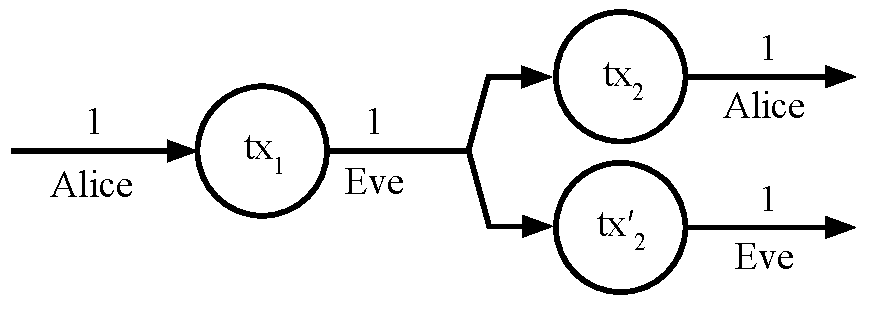
\includegraphics[width=0.6 \columnwidth,keepaspectratio]{figures/double-spend.pdf}
    \caption{A double spend transaction. Alice paid Eve $1$ unit through $\tx_1$, but Eve spent it in both $\tx_2$ and in $\tx_2'$,
             which have different recipients.}
    \label{fig.double-spend}
\end{figure}

\section{Simple Ideas Don't Work}

Let us consider three simple ideas to resolve the double spending problem that first come to mind.
Sadly, these ideas won't work.

\noindent
\textbf{Idea 1: Reject double spends altogether.} Honest parties never double spend. Since the adversary is the only one
creating double spends, why do we need to provide any assurances? We can opt to simply invalidate that
money. We add the following rule to our protocol:

\begin{quote}
If you see a transaction that is a double-spend,
then consider \emph{all} of the transaction outputs that pertain to the double spend transactions invalid.
\end{quote}

This approach is problematic. The reason is that the adversary can retroactively take back
a payment: She initially broadcasts $\tx_2$ to the network paying Alice, but keeps $\tx_2'$ withheld,
as illustrated in the timeline of Figure~\ref{fig.simple-idea-1}.
Alice, like everyone else, observes $\tx_2$ on the network, but not $\tx_2'$. She thinks this is
a normal transaction and accepts the payment. In exchange for this payment, Alice provides a service
to Eve: she serves her coffee. At a later time, Eve has enjoyed the coffee and has departed from Alice's
establishment. At this point, Eve broadcasts $\tx_2'$, a double spend of $\tx_2$. Suddenly, everyone
on the network considers both $\tx_2$ and $\tx_2'$ invalid. Alice's money is gone. Therefore, we cannot
adopt this construction.

\begin{figure}[h]
    \centering
    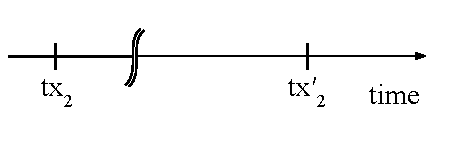
\includegraphics[width=0.4 \columnwidth,keepaspectratio]{figures/simple-idea-1.pdf}
    \caption{The first idea is unviable because it allows the
    adversary to retroactively invalidate an earlier transaction much later. Here, $\tx_2'$
    is initially withheld, but broadcast much later, causing an invalidation to the earlier
    $\tx_2$ transaction.}
    \label{fig.simple-idea-1}
\end{figure}

\noindent
\textbf{Idea 2: Accept the first transaction seen.} As we saw, two different honest parties can disagree in
the order in which two transactions arrived on the network. The situation is illustrated in
Figure~\ref{fig.simple-idea-2}. Therefore, the following simple construction does not work:

\begin{quote}
  Among double spending transactions, accept the first, and reject every subsequent transaction.
\end{quote}

However, we now note that these two transactions must be broadcast
to honest parties in close succession, and in particular within time $\Delta$. If the adversary
were to reveal $\tx_2$ to Charlie first, but then wait for more than $\Delta$ time until she revealed
$\tx_2'$ to Dave, then Charlie would have gossiped $\tx_2$ and Dave would have receive it within $\Delta$
and prior to seeing $\tx_2'$. In that case, Charlie and Dave would be in agreement.
In order for the adversary to cause disagreement, she must broadcast the two double spending
transactions to two different honest parties within time $\Delta$ of each other. Yet, this is
simple for an adversary to do, so we cannot adopt this construction either.

\begin{figure}[h]
    \centering
    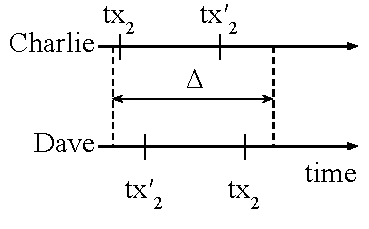
\includegraphics[width=0.325 \columnwidth,keepaspectratio]{figures/simple-idea-2.pdf}
    \caption{The second idea is unviable because parties
    have views in disagreement about transaction order. Here, Charlie believes $\tx_2$
    precedes $\tx_2'$, whereas Dave believes $\tx_2'$ precedes $\tx_2$.}
    \label{fig.simple-idea-2}
\end{figure}

\noindent
\textbf{Idea 3: Reject double spends within $u$.} Why don't we combine ideas 1 and 2? We saw that
Idea 1 is problematic because it allows the adversary to retroactively take back a transaction after
a long time into the future. We also saw that Idea 2 is problematic because it allows an adversary to
cause disagreement when two transactions are broadcast in close succession. This creates a natural
new construction idea:

\begin{quote}
Upon seeing a transaction, wait for some time $u \geq \Delta$. If a double spend
appears within the window $u$, reject all double spending transactions. However, if $u$ has passed and we have
not seen any double spends, accept the single transaction that we have seen. If a double spend appears in
the future, just reject that one.
\end{quote}

At first sight, this third idea seems to work: After time $u$ has passed, either the money is accepted or not.
The adversary cannot walk away as she did against Idea 1. If the adversary broadcasts two conflicting
transactions within $\Delta$ time, as she did against Idea 2, they will both be rejected. It won't matter
that different parties saw them in different order.

Sadly, on closer inspection, this idea does not work,
either. The strategy of the adversary is now to cause disagreement between Charlie and Dave with
regards to \emph{whether or not} the two transactions appeared within time $u$. The problematic situation
is illustrated in Figure~\ref{fig.simple-idea-3}. The adversary initially broadcasts $\tx_2$
to both Charlie and Dave. Both Charlie's and Dave's clocks start ticking to measure the time $u$.
Right before time $u$ hits, the adversary broadcasts $\tx_2'$ to Charlie. Now, Charlie has seen
a double spend within time $u$, and so he rejects both $\tx_2$ and $\tx_2'$. He also rebroadcasts
$\tx_2'$ to Dave, but this message will require time $\Delta$ to reach Dave. In the meantime,
time $u$ has passed, and Dave accepts $\tx_2$. When $\tx_2'$ arrives on Dave's end, Dave has
already accepted $\tx_2$ and now rejects $\tx_2'$. Now Charlie and Dave are in disagreement:
Dave thinks $\tx_2$ is valid, whereas Charlie thinks $\tx_2$ is invalid.

\begin{figure}[h]
    \centering
    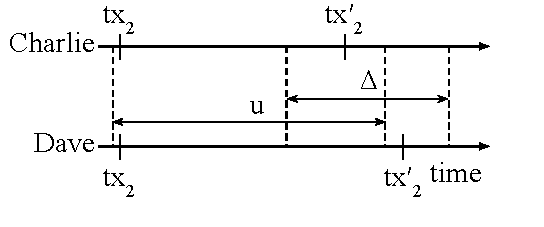
\includegraphics[width=0.45 \columnwidth,keepaspectratio]{figures/simple-idea-3.pdf}
    \caption{The third idea is unviable because parties
    disagree about whether $\tx_2$ and $\tx_2'$ have arrived within time $u$,
    and follow different policies. Here, Charlie rejects both transactions, whereas
    Dave accepts $\tx_2$ and rejects $\tx_2'$.}
    \label{fig.simple-idea-3}
\end{figure}

\section{Blocks and Blockchains}
\subsection{Virtues of Ledgers}
There are two virtues of ledgers that should be satisfied:
\begin{itemize}
    \item \textbf{Safety:} honest parties should agree and achieve consensus.
    \item \textbf{Liveness:} transactions created by honest parties are added to the ledgers of honest parties "soon".
\end{itemize}

As observed from previous examples, double spends occur because network delays can cause disagreements in the arrival time of different transactions. If somehow transactions could only be created in intervals greater than the network delay parameter $\Delta$, there would be no disagreements because each transaction would have already been broadcasted to all honest parties before the next one gets broadcasted. This gives rise to safety. However, requiring such a delay between transactions means that there will be less transactions being broadcasted every time period, and as such it may be the case that the liveness property is not satisfied. This presents a tradeoff between safety and liveness: as $\Delta$ increases, there is less certainty for liveness to be guaranteed.

\subsection{Blocks}

One way to satisfy both the virtues of safety and liveness is to group multiple transactions together and then broadcast them as "blocks", rather than individually. Each block, denoted $\Bar{x} = (tx_1, tx_2, \dots)$, contains a sequence of transactions in any order that respects the topological sorting of the corresponding UTXO graph.

In this model, double spends can only occur if the two transactions that creates the double spend exist in 2 different blocks that arrives in different order to different honest parties, similar to the previous example with transactions. If the two double spending transactions appeared within the same block, then there is no valid UTXO graph for the transactions of that block, and so the entire block is invalid. If the two double spending transactions appear in two blocks that are further than $\Delta$ apart, then the first transaction would have been validated by all honest parties, and so the second transaction fails to double spend.

Hence, all we need to do to ensure protection against double spending is to ensure that each  \textbf{block}—rather than each transaction—is rare, which preserves safety  while ensuring a higher level of liveness.

\begin{figure}[H]
    \centering
    \pgfplotsset{compat=1.15}


\tikzset{every picture/.style={line width=0.75pt}} %set default line width to 0.75pt

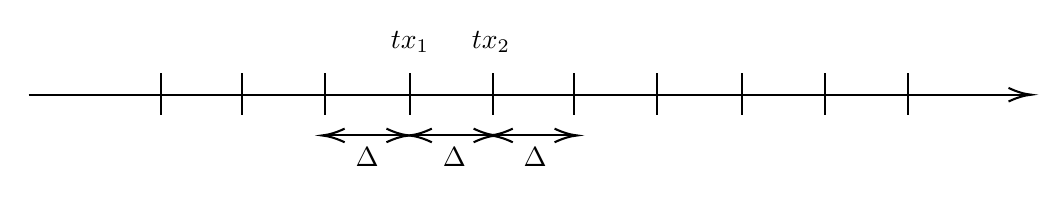
\begin{tikzpicture}[x=0.75pt,y=0.75pt,yscale=-1,xscale=1]
%uncomment if require: \path (0,300); %set diagram left start at 0, and has height of 300

%Straight Lines [id:da9017954087564621]
\draw    (97,110.2) -- (578,110.2) ;
\draw [shift={(580,110.2)}, rotate = 180] [color={rgb, 255:red, 0; green, 0; blue, 0 }  ][line width=0.75]    (10.93,-3.29) .. controls (6.95,-1.4) and (3.31,-0.3) .. (0,0) .. controls (3.31,0.3) and (6.95,1.4) .. (10.93,3.29)   ;
%Straight Lines [id:da09295967444550124]
\draw    (160.73,99.83) -- (160.73,119.83) ;
%Straight Lines [id:da22506827825676345]
\draw    (199.73,99.83) -- (199.73,119.83) ;
%Straight Lines [id:da6864589596901391]
\draw    (239.73,99.83) -- (239.73,119.83) ;
%Straight Lines [id:da3375627515094475]
\draw    (280.73,99.83) -- (280.73,119.83) ;
%Straight Lines [id:da2711314265282385]
\draw    (320.73,99.83) -- (320.73,119.83) ;
%Straight Lines [id:da9006595698348807]
\draw    (359.73,99.83) -- (359.73,119.83) ;
%Straight Lines [id:da2941667702377173]
\draw    (399.73,99.83) -- (399.73,119.83) ;
%Straight Lines [id:da4637768077817921]
\draw    (440.73,99.83) -- (440.73,119.83) ;
%Straight Lines [id:da15003143298927957]
\draw    (480.73,99.83) -- (480.73,119.83) ;
%Straight Lines [id:da7785431556267932]
\draw    (520.73,99.83) -- (520.73,119.83) ;
%Straight Lines [id:da07195865234652721]
\draw    (259.29,129.83) -- (278.29,129.83) ;
\draw [shift={(280.29,129.83)}, rotate = 180] [color={rgb, 255:red, 0; green, 0; blue, 0 }  ][line width=0.75]    (10.93,-3.29) .. controls (6.95,-1.4) and (3.31,-0.3) .. (0,0) .. controls (3.31,0.3) and (6.95,1.4) .. (10.93,3.29)   ;
%Straight Lines [id:da13395559951976144]
\draw    (259.29,129.83) -- (240.29,129.83) ;
\draw [shift={(238.29,129.83)}, rotate = 360] [color={rgb, 255:red, 0; green, 0; blue, 0 }  ][line width=0.75]    (10.93,-3.29) .. controls (6.95,-1.4) and (3.31,-0.3) .. (0,0) .. controls (3.31,0.3) and (6.95,1.4) .. (10.93,3.29)   ;
%Straight Lines [id:da3690305468137254]
\draw    (301.29,129.83) -- (320.29,129.83) ;
\draw [shift={(322.29,129.83)}, rotate = 180] [color={rgb, 255:red, 0; green, 0; blue, 0 }  ][line width=0.75]    (10.93,-3.29) .. controls (6.95,-1.4) and (3.31,-0.3) .. (0,0) .. controls (3.31,0.3) and (6.95,1.4) .. (10.93,3.29)   ;
%Straight Lines [id:da6757384410639338]
\draw    (301.29,129.83) -- (282.29,129.83) ;
\draw [shift={(280.29,129.83)}, rotate = 360] [color={rgb, 255:red, 0; green, 0; blue, 0 }  ][line width=0.75]    (10.93,-3.29) .. controls (6.95,-1.4) and (3.31,-0.3) .. (0,0) .. controls (3.31,0.3) and (6.95,1.4) .. (10.93,3.29)   ;
%Straight Lines [id:da008698697312877313]
\draw    (340.29,129.83) -- (359.29,129.83) ;
\draw [shift={(361.29,129.83)}, rotate = 180] [color={rgb, 255:red, 0; green, 0; blue, 0 }  ][line width=0.75]    (10.93,-3.29) .. controls (6.95,-1.4) and (3.31,-0.3) .. (0,0) .. controls (3.31,0.3) and (6.95,1.4) .. (10.93,3.29)   ;
%Straight Lines [id:da5776529929797669]
\draw    (340.29,129.83) -- (321.29,129.83) ;
\draw [shift={(319.29,129.83)}, rotate = 360] [color={rgb, 255:red, 0; green, 0; blue, 0 }  ][line width=0.75]    (10.93,-3.29) .. controls (6.95,-1.4) and (3.31,-0.3) .. (0,0) .. controls (3.31,0.3) and (6.95,1.4) .. (10.93,3.29)   ;

% Text Node
\draw (253,134.4) node [anchor=north west][inner sep=0.75pt]    {$\Delta $};
% Text Node
\draw (295,134.4) node [anchor=north west][inner sep=0.75pt]    {$\Delta $};
% Text Node
\draw (334,134.4) node [anchor=north west][inner sep=0.75pt]    {$\Delta $};
% Text Node
\draw (270,78.4) node [anchor=north west][inner sep=0.75pt]    {$tx_{1}$};
% Text Node
\draw (309,78.4) node [anchor=north west][inner sep=0.75pt]    {$tx_{2}$};


\end{tikzpicture}

    \caption{In an ideal scenario, each blocks are broadcasted exactly $\Delta$ away from each other, so in a double spend we can always accept $tx_1$ and reject $tx_2$}
    \label{fig:my_label}
\end{figure}

\subsection{Proof of Work and Mining}
To ensure that the ability to create blocks is rare (i.e. that one can only be created after $\Delta$ has passed since the last block), we devise a scheme to issue rare tickets for creating a block. To do so, we will introduce the concept of Proof of Work.

% \subsection{Blocks and Proof of Work}

% There are two virtues of ledgers. The first is safety, which means that ledgers of honest parties should agree and reach consensus. The second is liveness, which means a transaction issued by an honest party should make it into honest ledgers soon.

% As observed from previous examples, a reason why double spends are difficult to deal with is because two transactions can be broadcasted within a short time span. If only one transaction can be broadcasted every $\Delta$, then the problem of double spends is easy to deal with because each node would receive transactions in the same order. However, the tradeoff in this case would slow throughput which can prevent the liveness property from being satisfied.

% This motivates the use of blocks to store transactions. A block stores a bundled sequence of transactions, denoted as $\Bar{x}$. We want one new block to be broadcasted roughly every $\Delta$. To ensure this time span, we will introduce the Proof-of-Work Equation.

\begin{definition}[Proof-of-Work Equation]
  $H(B) \leq T$
  \footnote{This scheme was derived in 1993 by Cynthia Dwork and Moni Naor in the seminal paper "Pricing via Processing
or Combatting Junk Mail".}
\end{definition}

Here, $T$ is called the target. In order to solve the Proof-of-Work equation, one would have to find a value of $B$ such that $H(B) \leq T$.

\begin{definition}[Random Oracle Model]
  Output of $H$ is distributed uniformly at random.
\end{definition}

Under the Random Oracle Assumption, notice that the time it would take to find a bruteforce solution to a Proof-of-Work equation depends on the value of $T$. When $T$ is larger, it would be easier to find $B$ such that $H(B) \leq T$, and vice versa. In particular, $Pr[H(B) \leq T] = \frac{T}{2^{\kappa}}$ for any arbitrary $B$.

In the network, $T$ is fixed and hard-coded for honest parties. The value is chosen such that the time it takes for a node in the network to find a solution to the Proof-of-Work equation is around $\Delta$.

Now, notice that if we allow honest parties to pick whatever $B$ they want, then as soon as the first valid value of $B$ is found, each node can just trivially reuse that value instantaneously, and safety is lost again. As such, in the network, we require that $B = \delta||\Bar{x}||ctr$, where $||$ means concatenation and where $\delta$ is the hash of the previous block $H(B')$. Both $\delta$ and $\Bar{x}$ are fixed, and $ctr$ is a number to be found that solves the Proof-of-Work equation. In other words, when nodes are trying to solve the Proof-of-Work equation, they are trying different values of $ctr$ until finding a satisfactory one. The time it takes the first node to find a satisfactory $ctr$ for their block will be around $\delta$. The process of finding a bruteforce solution to the Proof-of-Work equation is called mining.

\subsection{Blockchains}

The previous block hash, $\delta$, is a part of $B$ because we want to ensure "freshness", which means that only blocks that are recently created should be able to be broadcasted. Consider the scenario where an adversary mines multiple blocks, but does not broadcast them immediately. Then, at a later point in time, the adversary broadcast all of these blocks at the same time. Since there is not a $\Delta$ interval between the time these blocks are broadcasted, the problem of double spend arises again. There could be disagreements in the ledgers of the honest nodes. In order to prevent this, we require each block to point to the most recent known block. By including $\delta$ as a part of $B$, we ensure that blocks that were mined beforehand are no longer valid, since the adversary could not have predicted $\delta$ before the most recent block was broadcasted. As a result, we can guarantee that blocks will be roughly be broadcasted in regular time intervals. Since blocks are all connected to each other in this way, this chain of block is called the \emph{blockchain}.


\subsection{Genesis Block}

The Genesis Block is the first block in a blockchain. It contains real world data to anchor time, in order to ensure that it is impossible to pre-mine. If the hash of the Genesis Block is known before it is broadcasted, then the adversary could pre-mine multiple blocks beforehand (before the network is even available to the rest of the world). Then, when the Genesis Block is broadcasted, the adversary would be able to broadcast multiple blocks within a short time span. Hence, it is necessary for the Genesis Block to contain real world data to anchor time. For example, Bitcoin genesis block quotes the January 3  2009 The Times headline.

\begin{figure}[H]
    \centering
    \pgfplotsset{compat=1.15}



\tikzset{every picture/.style={line width=0.75pt}} %set default line width to 0.75pt

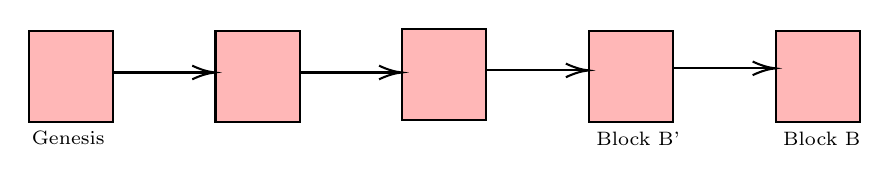
\begin{tikzpicture}[x=0.75pt,y=0.75pt,yscale=-1,xscale=1]
%uncomment if require: \path (0,165); %set diagram left start at 0, and has height of 165

%Shape: Rectangle [id:dp6459725379232777]
\draw  [fill={rgb, 255:red, 255; green, 183; blue, 183 }  ,fill opacity=1 ] (132,36) -- (172.53,36) -- (172.53,80.09) -- (132,80.09) -- cycle ;
%Shape: Rectangle [id:dp7451543919622989]
\draw  [fill={rgb, 255:red, 255; green, 183; blue, 183 }  ,fill opacity=1 ] (222,36) -- (262.53,36) -- (262.53,80.09) -- (222,80.09) -- cycle ;
%Shape: Rectangle [id:dp4942977774139823]
\draw  [fill={rgb, 255:red, 255; green, 183; blue, 183 }  ,fill opacity=1 ] (312,35) -- (352.53,35) -- (352.53,79.09) -- (312,79.09) -- cycle ;
%Shape: Rectangle [id:dp8525801453597799]
\draw  [fill={rgb, 255:red, 255; green, 183; blue, 183 }  ,fill opacity=1 ] (402,36) -- (442.53,36) -- (442.53,80.09) -- (402,80.09) -- cycle ;
%Shape: Rectangle [id:dp16781400895186005]
\draw  [fill={rgb, 255:red, 255; green, 183; blue, 183 }  ,fill opacity=1 ] (492,36) -- (532.53,36) -- (532.53,80.09) -- (492,80.09) -- cycle ;
%Straight Lines [id:da27296871485376917]
\draw    (172.73,56.09) -- (219.73,56.09) ;
\draw [shift={(221.73,56.09)}, rotate = 180] [color={rgb, 255:red, 0; green, 0; blue, 0 }  ][line width=0.75]    (10.93,-3.29) .. controls (6.95,-1.4) and (3.31,-0.3) .. (0,0) .. controls (3.31,0.3) and (6.95,1.4) .. (10.93,3.29)   ;
%Straight Lines [id:da8965885073779516]
\draw    (262.73,56.09) -- (309.73,56.09) ;
\draw [shift={(311.73,56.09)}, rotate = 180] [color={rgb, 255:red, 0; green, 0; blue, 0 }  ][line width=0.75]    (10.93,-3.29) .. controls (6.95,-1.4) and (3.31,-0.3) .. (0,0) .. controls (3.31,0.3) and (6.95,1.4) .. (10.93,3.29)   ;
%Straight Lines [id:da16101344176853494]
\draw    (352.73,55.09) -- (399.73,55.09) ;
\draw [shift={(401.73,55.09)}, rotate = 180] [color={rgb, 255:red, 0; green, 0; blue, 0 }  ][line width=0.75]    (10.93,-3.29) .. controls (6.95,-1.4) and (3.31,-0.3) .. (0,0) .. controls (3.31,0.3) and (6.95,1.4) .. (10.93,3.29)   ;
%Straight Lines [id:da6603043582779935]
\draw    (442.73,54.09) -- (489.73,54.09) ;
\draw [shift={(491.73,54.09)}, rotate = 180] [color={rgb, 255:red, 0; green, 0; blue, 0 }  ][line width=0.75]    (10.93,-3.29) .. controls (6.95,-1.4) and (3.31,-0.3) .. (0,0) .. controls (3.31,0.3) and (6.95,1.4) .. (10.93,3.29)   ;

% Text Node
\draw (132,83.09) node [anchor=north west][inner sep=0.75pt]   [align=left] {{\scriptsize Genesis}};
% Text Node
\draw (404,83.09) node [anchor=north west][inner sep=0.75pt]   [align=left] {{\scriptsize Block B'}};
% Text Node
\draw (494,83.09) node [anchor=north west][inner sep=0.75pt]   [align=left] {{\scriptsize Block B}};


\end{tikzpicture}

    \caption{To mine block B, the miner runs the Proof of Work Equation with B = $H(B')||\Bar{x}||ctr$}
    \label{fig:my_label}
\end{figure}


\subsection{Honest Party Block Generation Algorithm}

Putting it all together, an honest party (which we can assume to be every honest node in the network for now) follows the following algorithm to create a valid block. First, it collects any amount of transactions from the network and add them to a mempool, which is a set of validated but unconfirmed transactions \footnote{The number of transactions it collects will be formalized later}. Then, it writes $B = \delta||\Bar{x}||ctr$, and then solves the Proof-of-Work Equation. In other words, it finds a value of ctr (which is also known as the nonce) such that $H(B) \leq T$. If the honest party is successful, it will broadcast the mined block to the network. Otherwise, if another block has been found and received by the honest party first, it will validate the new block, update it's UTXO by removing all the transactions that were spent in the newest block, and update the freshest block in its memory. As such, $B$ would necessarily change, and the honest party will have to solve a new Proof-of-Work equation.

%TODO: maybe rewrite using algorithms package?
